\section{Durchführung}
\label{sec:durchfuehrung}

    Für die Durchführung des Versuches ist der folgende Aufbau gegeben.

    \begin{figure}
        \centering
        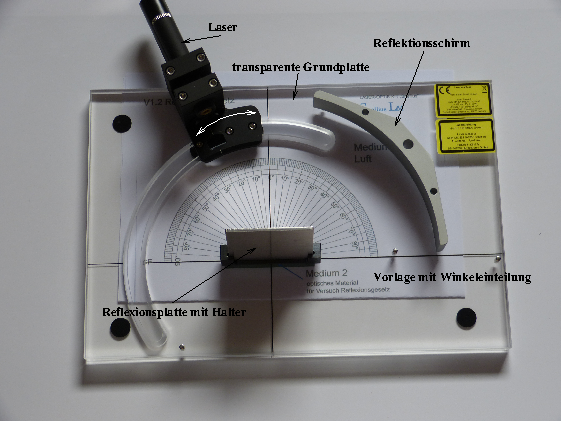
\includegraphics[width=\textwidth]{content/img/Abb_3.pdf}
        \caption{Der Gesamtaufbau des Versuchs. \cite{versuchsanleitung}}
        \label{fig:gesamtaufbau}
    \end{figure}

    Das Licht wird mithilfe einer Spektrallampe erzeut,
    in diesem Fall einer Quecksilberdampflampe,
    welche möglichst wenig an- und ausgeschaltet werden sollte.
    Der Lichtstrahl wird mithilfe einer Kondensatorlinse und einer Spaltblende gebündelt.
    Die Abbildungslinse beeinflusst die Form des Lichtstrahls und passt sie der Spaltblende an.
    Mithilfe des Prismas wird das Licht in seine verschiedenen Wellenlängen aufgespalten,
    sodass nur ein schmaler Wellenlängenbereich auf die Photokathode trifft,
    wobei die verwendete Photozelle der in \autoref{fig:aufbau_photozelle} dargestellten entspricht.
    Das aufgespaltene Licht kann auf einem Leuchtschirm oder einem Blatt Papier,
    welches vor die Photozelle gehalten wird,
    sichtbar gemacht werden.\\

    \begin{figure}[H]
        \centering
        \includegraphics[width=0.5\textwidth]{content/img/Abb_2_edit.pdf}
        \caption{Schematische Darstellung der verwendeten Photozelle. \cite{versuchsanleitung}}
        \label{fig:aufbau_photozelle}
    \end{figure}

    Zur Messung des Photostroms ist die Apparatur in der folgenden \autoref{fig:schaltbild} gegeben.

    \begin{figure}[H]
        \centering
        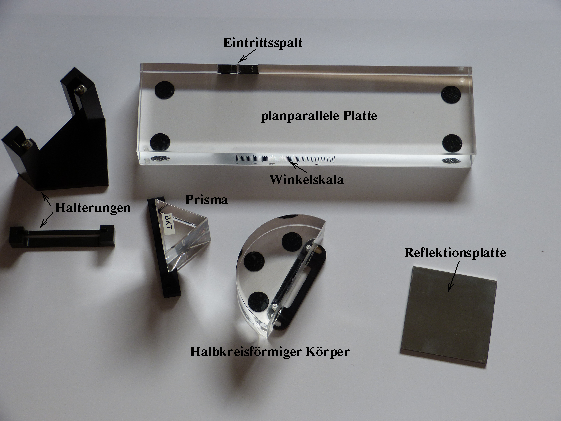
\includegraphics[width=0.6\textwidth]{content/img/Abb_4.pdf}
        \caption{Schaltbild zur Messung des Photostroms $I_\text{Ph}$ und Aufbau einer Spannung $U$. \cite{versuchsanleitung}}
        \label{fig:schaltbild}
    \end{figure}

    % https://tex.stackexchange.com/a/78017
    \phantomsection
    \label{sec:durchfuehrung:dunkelstrom}
    Zu Beginn der Messung wird der sogenannte Dunkelstrom gemessen,
    also der Strom,
    der durch Umgebungslicht erzeugt wird.
    Dazu wird das Prisma verdeckt,
    indem ein Gegenstand zwischen Prisma und Photozelle gehalten wird,
    und der Strom auf dem Messgerät abgelesen.\\
    Anschließend werden die optischen Instrumente so eingestellt,
    dass sich ein möglichst scharfes Bild der einzelnen Linien ergibt.
    \\
    Es werden nun nacheinander verschiedene Linien des aufgespaltenen Lichts auf den Eingang der Photozelle gerichtet,
    wozu der Schwenkarm verwendet wird.
    Dabei muss darauf geachtet werden,
    dass das empfindliche Koaxialkabel,
    über welches die Photozelle mit dem Strommessgerät verbunden ist,
    nicht zu stark bewegt wird.
    Für etwa drei bis vier Linien wird in einem Intervall von $\SI{- 5}{\volt}$,
    also einer beschleunigenden Spannung,
    bis $\SI{5}{\volt}$,
    einer bremsenden Spannung,
    der Wert für den Photostrom $I_\text{Ph}$ gemessen.
    \\
    Für die gelbe Linie mit der Wellenlänge $\lambda = \SI{578}{\nano\meter}$
    wird zusätzlich ein größerer Bereich von
    $\SI{- 20}{\volt}$ bis $\SI{20}{\volt}$ gemessen.\\
    Zwischen den Messungen der Linien muss gegebenenfalls das Bild erneut scharf gestellt werden.
